\documentclass[12pt,fleqn]{article}
\usepackage{../lecture-notes/vkCourseML}
\usepackage{lipsum}
\usepackage{indentfirst}
\usepackage{graphicx}
\usepackage{animate}
\usepackage{hyperref}
\graphicspath{{./figures/}}
\title{Машинное обучение, ФКН ВШЭ\\Семинар №4\\Предобработка данных}
\author{}
\date{}

\begin{document}
\maketitle


\section{Пропущенные значения}

В реальных задачах значения некоторых признаков у некоторых объектов отсутствуют. Это может происходить по разным причинам: ошибки при записи данных, отказ респондента отвечать на вопрос, невозможность описать конкретное свойство у конкретного объекта (в таблице с данными об автомобилях будут пропуски у электромобилей в графе <<объём топливного бака>>). Многие алгоритмы машинного обучения (в частности, линейная регрессия) не могут работать с пропущенными данными, поэтому эти пропуски необходимо заполнить.

Заполнять пропуски у объектов можно различными способами:
\begin{enumerate}
  \item Константным уникальным значением "--- неудачный вариант для линейных методов (модель начнёт считать пропуск близким к некоторому другому значению выборки), но быстрый и популярный способ с другими алгоритмами в машинном обучении.
  \item Средним арифметическим, медианой, модой "--- сохранение статистик выборки, но потеря информации о наличии пропуска в данных.
  \item Предсказаниями другого алгоритма "--- затратно по времени (однако всё равно не приносит новой информации в датасет, хотя и может положительно сказаться на общем качестве).
\end{enumerate}

Заметим, что в некоторых случаях наличие пропуска в данных несёт определённую информацию об объекте (например, отказ в ответе на вопрос о доходах клиента банка), поэтому полезно добавлять новые признаки "--- индикаторы пропусков. Иногда признаки содержат слишком много пропусков и их выгоднее удалить.

Добавление индикаторов пропусков даёт интересную возможность. Допустим, у нас встречаются пропуски в признаке~$x_1$,
и мы добавляем второй признак с соответствующим индикатором:
\[
    a(x)
    =
    w_0
    +
    w_1 x_1
    +
    w_2 [\text{был пропуск в} x_1]
    +
    \dots
\]
Заметим, что если мы заменяем пропуски в~$x_1$ на какую-то константу, то~$w_2$, по сути, может скорректировать эту константу.
Получается, что добавление индикатора позволяет выучить оптимальную константу для замены пропусков.

\section{Выбросы}


На практике могут встречаться объекты, сильно отличающиеся от остальных. Их называют выбросами. Отличия могут выражаться как в значениях признаков, так и в целовой величине. Причины бывают различными: ошибки в заполнении данных (добавили лишний ноль), <<исключительность>> отдельных объектов (низкие цены на дома могут быть связаны с попыткой обхода налогов, а не с их характеристиками). Выбросы могут сильно сказываться на решении "--- например, квадратичная функция ошибок <<реагирует>> на выбросы и линейная регрессия с таким функционалом ошибки отклоняется в их сторону, в отличие от модели, оптимизирующей среднюю абсолютную ошибку (рис. \ref{fig:outliers}).

\begin{center}
    \begin{figure}[!htb]
        \centering
        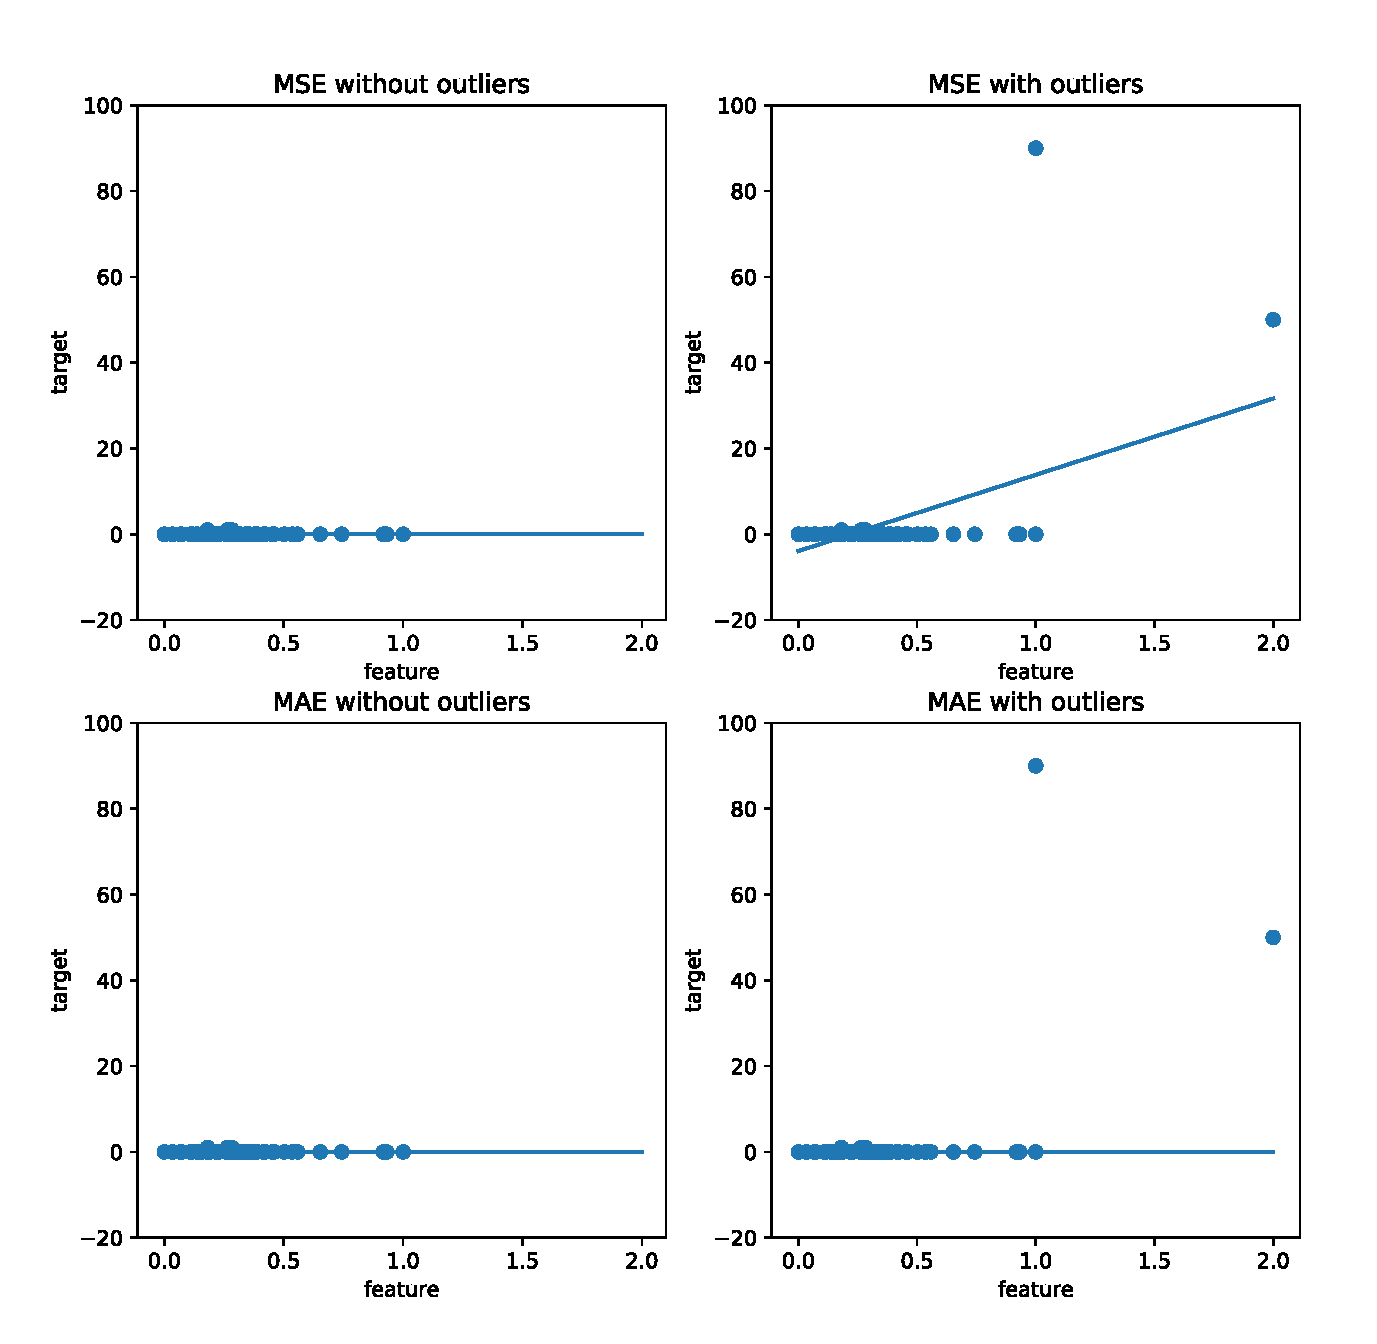
\includegraphics[width=0.8\linewidth]{img/outliers.eps}
        \caption{Влияние выбросов на обученную линейную регрессию для MSE и MAE в качестве функции потерь.}\label{fig:outliers}
    \end{figure}
\end{center}

Искать выбросы можно следующим образом. Выбросы в признаках можно обнаружить, исследуя распределение признаков и в особенности хвосты распределений. Выбросы в целевой величине можно искать, считая ошибку предсказания модели на объектах обучающей выборки (вспомогательная модель не должна наблюдать при обучении проверяемый объект). Если ошибка велика (алгоритм с уверенностью предсказывает отрицательный класс, хотя метка у объекта положительная), то объект можно считать выбросом (если, конечно, дело не в плохой модели). Объекты-выбросы чаще всего не корректируют, а удаляют из выборки.

Заметим, что не всегда необходимо удалять объекты-выбросы из выборки. В одном \href{https://habr.com/company/ods/blog/336168/}{конкурсе} помог следующий подход: оставить выбросы, чтобы не изменилось среднее предсказание алгоритма, при этом качество модели считать только по <<нормальным>> объетам, чтобы исключить шум от объектов-выбросов.

Как уже было сказано выше, некоторые функции потерь чувствительнее относятся в выбросам, поэтому в таких ситуациях имеет смысл использовать более устойчивые функции потерь для обучения моделей.

\section{Обработка категориальных признаков}

Часто в данных встречаются категориальные по смыслу признаки. Если они представлены в виде чисел, то, подавая напрямую в модель, мы задаём порядок над этими категориями, что обычно неправильно. Например, если красный цвет кодировался как <<1>>, зелёный "--- <<2>>, а синий "--- <<3>>, то модель будет считать зелёный цвет находящимся ровно между красным и синим. Если же категориальный признак представлен в выборке не в виде чисел, то мы и вовсе не можем использовать его для обучения модели. Изучим способы кодирования категориальных признаков.

\subsection{Label encoding}

В простом случае, если категориальный признак представлен в виде нечисловых данных, можно построить обратимое отображение для каждого уникального значения в некоторое число. Это позволит использовать признак для обучения модели. Например, зелёному цвету будет соответствовать <<1>>, красному "--- <<2>> и так далее.

У этого подхода две основные проблемы: задание порядка над категориями и работа с неизвестными в процессе обучения значениями категориального признака (нужно не забывать обрабатывать такой случай отдельно).

\subsection{One-hot encoding}

Другой способ кодирования заключается в добавлении признаков-индикаторов категориальных значений. Например, появятся новые бинарные признаки: <<красный цвет>>, <<зелёный цвет>> и так далее. В этом случае решается проблема с заданием порядка над категориями и новыми значениями категориального признака (у такого объекта просто будут <<нули>> по всем признакам индикаторам).

Проблема этого подхода в увеличении количества признаков (а это затрачиваемая память и скорость обучения модели) пропорционально количеству категорий. Эти разреженные признаки допускают хранение в виде разреженных матриц, но только некоторые алгоритмы умеют работать с ними. Также можно для экономии памяти не создавать признаки для редко встречающихся категорий.

\subsection{Кодирование с учётом целевой переменной}

Более сложный метод кодирования категориальных признаков "--- через целевую переменную.
Идея в том, что алгоритму для предсказания цены необходимо знать не конкретный цвет автомобиля,
а то, как этот цвет сказывается на цене.
Разберём сначала базовый подход~--- mean target encoding~(иногда его называют~<<счётчиками>>).

Заменим каждую категорию на среднее значение целевой переменной по всем объектам этой категории.
Пусть~$j$-й признак является категориальным.
Для бинарной классификации новый признак будет выглядеть следующим образом:
\begin{equation}
\label{eq:meantarget}
    g_j(x, X)
    =
    \frac{
        \sum_{i=1}^{\ell}
            [f_j(x) = f_j(x_i)][y_i = +1]
    }{
        \sum_{i=1}^{\ell}
            [f_j(x) = f_j(x_i)]
    },
\end{equation}
где $f_j(x_i)$ -- $j$-й признак $i$-го объекта, $y_i$ -- класс $i$-го объекта.

Отметим, что эту формулу легко перенести как на случай многоклассовой классификации~(в этом случае
будем считать~$K$ признаков, по одному для каждого класса, и в числителе будет подсчитывать долю
объектов с заданной категорией и с заданным классом),
так и на случай регрессии~(будем вычислять среднее значение целевой переменной среди объектов данной категории).

Вернёмся к бинарной классификации.
Можно заметить, что для редких категорий мы получим некорректные средние значения целевой переменной.
Например, в выборке было только три золотистых автомобиля, которые оказались старыми и дешёвыми.
Из-за этого наш алгоритм начнёт считать золотистый цвет дешёвым.
Для исправления этой проблемы можно регуляризировать признак средним значением целевой переменной по всем категориям так,
чтобы у редких категорий значение было близко к среднему по всей выборке,
а для популярных к среднему значению по категории.
Формально для задачи бинарной классификации это выражается так:
\begin{equation}
\label{eq:meantarget-reg}
    g_j(x, X)
    =
    \frac{
        \sum_{i=1}^{\ell}
            [f_j(x) = f_j(x_i)][y_i = +1]
            +
            \frac{C}{\ell}
            \sum_{i=1}^{\ell}
            [y_i = +1]
    }{
        \sum_{i=1}^{\ell}
        [f_j(x) = f_j(x_i)] + C
    },
\end{equation}
где $C$ -- коэффициент, отвечающий за баланс между средним значением по категории и глобальным средним значением.

Однако если мы вычислим значения $g_j(x, X)$ по всей выборке,
то столкнёмся с переобучением, так как мы внесли информацию о целевой переменной
в признаки~(новый признак слабая, но модель, предсказывающая целевое значение).
Поэтому вычисление таких признаков следует производить по блокам,
то есть вычислять средние значения на основе одних фолдов
для заполнения на другом блоке~(аналогично процессу кросс-валидации).
Если же ещё планируется оценка качества модели с помощью кросс-валидации по блокам,
то придётся применить <<двойную кросс-валидацию>> для подсчёта признаков.
Этот подход заключается в кодировании категориальных признаков по <<внутренним>> блокам внутри <<внешних>> блоков,
по которым оценивается качество модели.

Разберём этот процесс~(иллюстрация на рис.~\ref{fig:cv_meantarget}).
Представим, что хотим посчитать качество модели на 3-м блоке. Для этого:
\begin{enumerate}
    \item Разбиваем все внешние блоки, кроме 3-го, на внутренние блоки.
        Количество внутренних блоков может не совпадать с количеством внешних~(на иллюстрации их также 3).
    \item Рассмотрим конкретный внешний блок.
        Для каждого из его внутренних блоков считаем значение~$g(x, X)$ на основе средних значений целевой переменной по блокам,
        исключая текущий. Для 3-го внешнего блока~(который сейчас играет роль тестовой выборки)
        вычисляем~$g(x, X)$ как среднее вычисленных признаков по каждому из внутренних фолдов.
    \item Обучаем модель на всех блоках, кроме 3-го, делаем предсказание на 3-м и считаем на нём качество.
\end{enumerate}

\begin{center}
\begin{figure}[!htb]
 \centering
 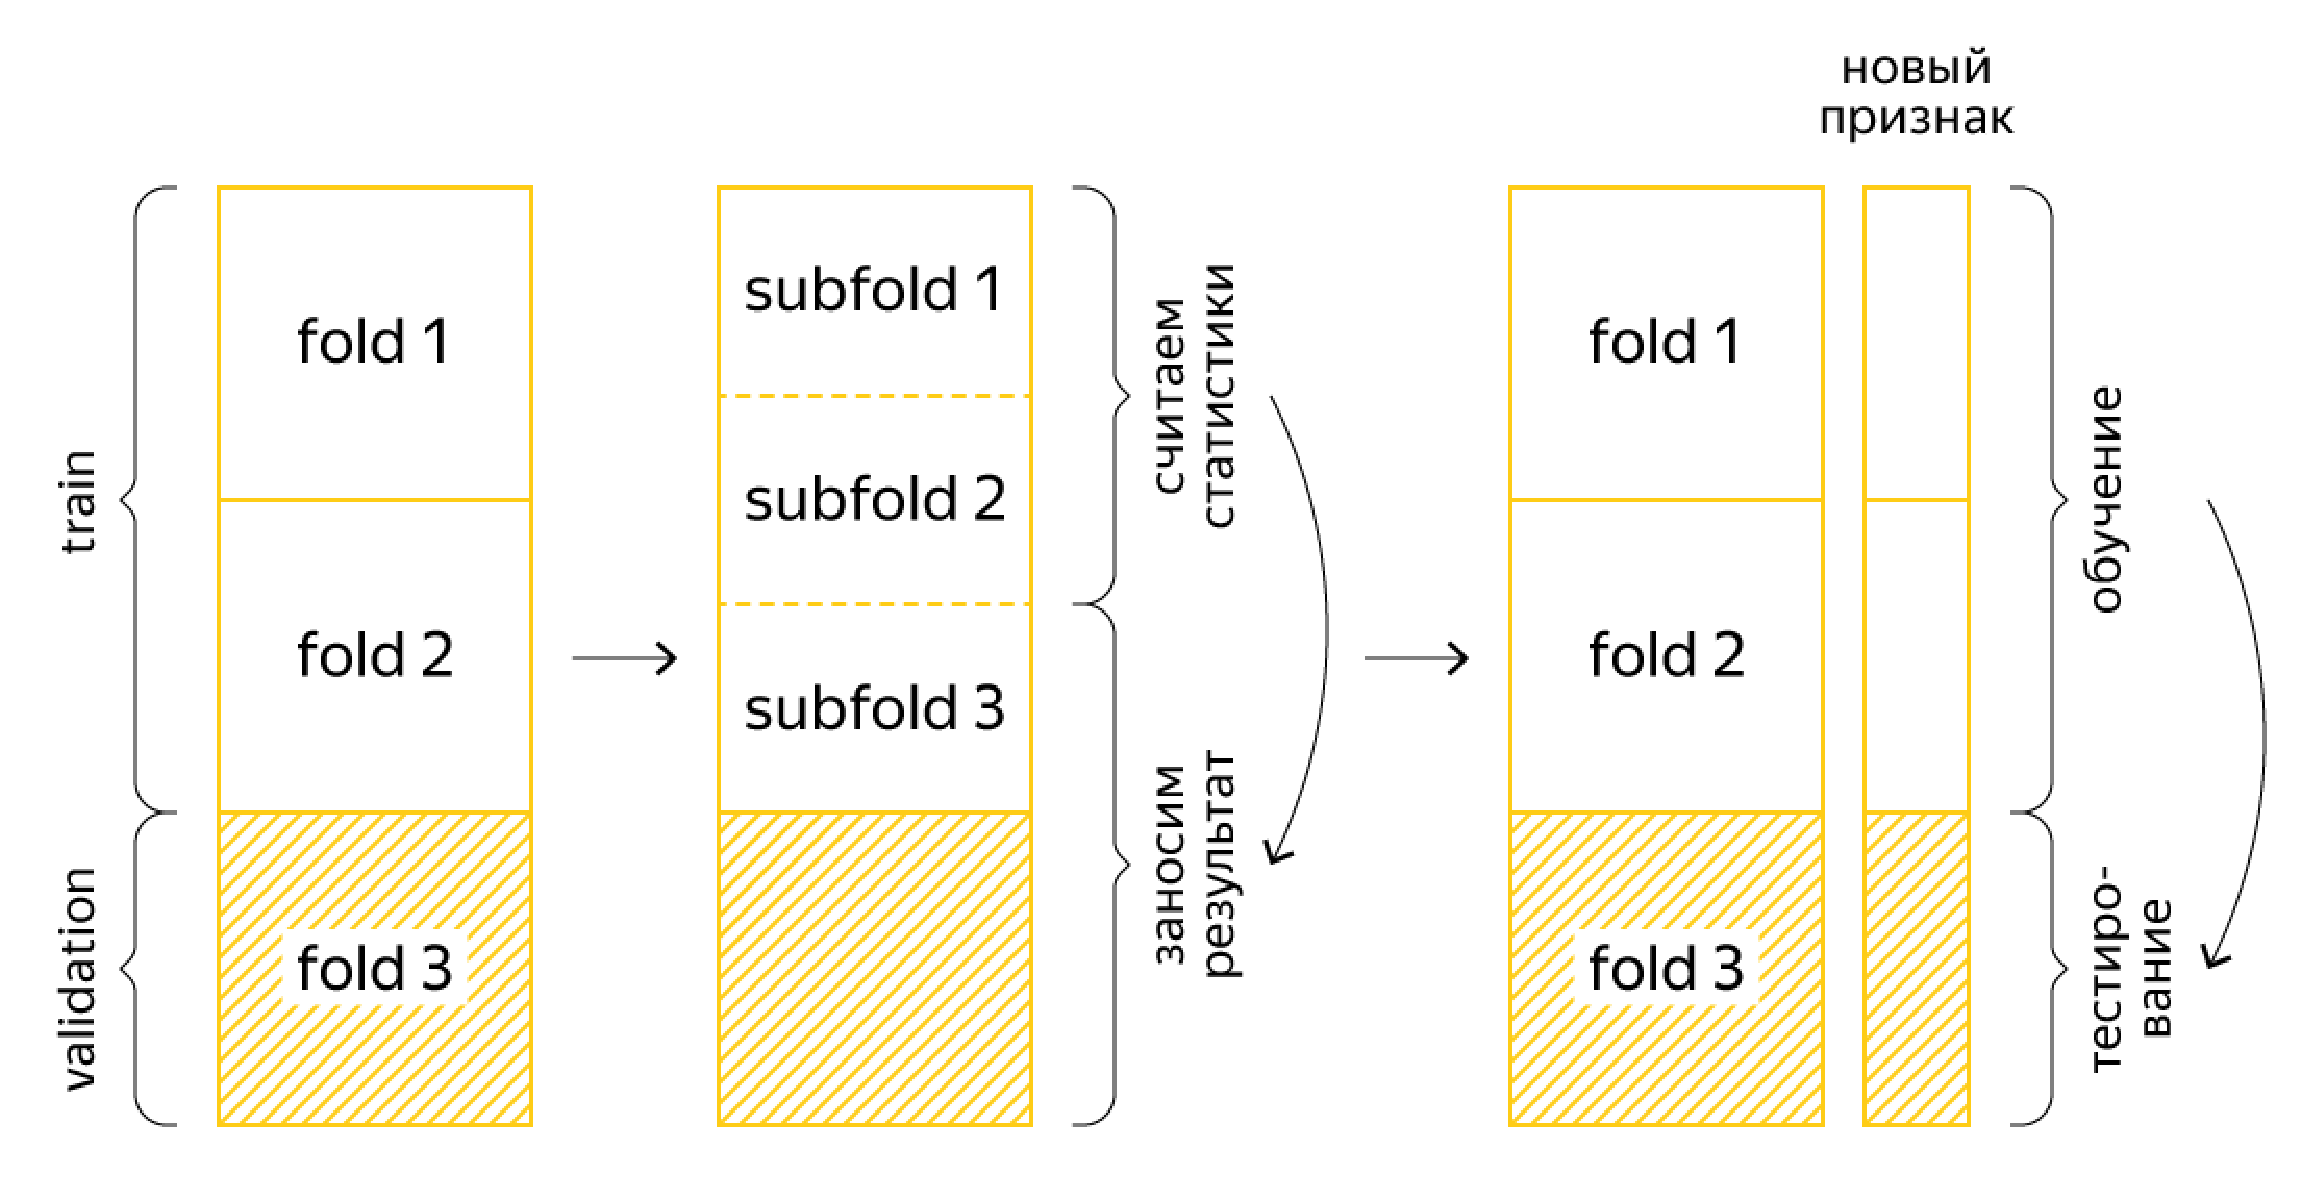
\includegraphics[width=0.8\linewidth]{img/cv_meantarget.eps}
 \caption{Кросс-валидация при кодировании средним значением}\label{fig:cv_meantarget}
\end{figure}
\end{center}

Существуют альтернативы кодированию категориальных признаков по блокам.

\paragraph{Зашумление.}
Можно посчитать новые признаки по базовой формуле~\eqref{eq:meantarget},
а затем просто добавить к каждому значению случайный шум~(например, нормальный).
Это действительно снизит уровень корреляции счётчиков с целевой переменной.
Проблема в том, что это делается за счёт снижения силы такого признака,
а значит, мы ухудшаем итоговое качество модели.
Поэтому важно подбирать дисперсию шума, чтобы соблюсти баланс между борьбой с переобучением
и предсказательной силой счётчиков.

\paragraph{Сглаживание.}
Можно немного модифицировать формулу~\eqref{eq:meantarget-reg},
чтобы сила регуляризации зависела от объёма данных по конкретной категории:
\begin{equation*}
    g_j(x, X)
    =
    \lambda \left( n(f_j(x)) \right)
    \frac{
        \sum_{i=1}^{\ell}
            [f_j(x) = f_j(x_i)][y_i = +1]
    }{
        \sum_{i=1}^{\ell}
        [f_j(x) = f_j(x_i)]
    }
    +
    \left( 1 - \lambda \left( n(f_j(x)) \right) \right)
    \frac{1}{\ell}
    \sum_{i = 1}^{\ell}
        [y_i = +1]
    ,
\end{equation*}
где~$n(z) = \sum_{i = 1}^{\ell} [f_j(x_i) = z]$~--- число объектов категории~$z$,
$\lambda(n)$~--- некоторая монотонно возрастающая функция, дающая значения из отрезка~$[0, 1]$.
Примером может служить~$\lambda(n) = \frac{1}{1 + \exp(-n)}$.
Если грамотно подобрать эту функцию, то она будет вычищать значение целевой переменной
из редких категорий и мешать переобучению.

\paragraph{Кодирование по времени.}
Можно отсортировать выборку некоторым образом и для~$i$-го объекта вычислять статистики только по предыдущим объектам:
\begin{equation*}
    g_j(x_k, X)
    =
    \frac{
        \sum_{i=1}^{k - 1}
            [f_j(x) = f_j(x_i)][y_i = +1]
    }{
        \sum_{i=1}^{k - 1}
            [f_j(x) = f_j(x_i)]
    }.
\end{equation*}
Для хорошего качества имеет смысл отсортировать выборку случайным образом несколько раз,
и для каждого такого порядка посчитать свои счётчики.
Это даёт улучшение качества, например, потому что для объектов, находящихся в начале выборки,
признаки будут считаться по очень небольшой подвыборке, и поэтому вряд ли будут хорошо предсказывать
целевую переменную.
При наличии нескольких перестановок хотя бы один из новых признаков будет вычислен по подвыборке
достаточного размера.
Такой подход, например, используется в библиотеке CatBoost.

\paragraph{Weight of Evidence.}
Существует альтернативный способ кодирования категориальных признаков, основанный на подсчёте соотношения
положительных и отрицательных объектов среди объектов данной категории.
Этот подход, в отличие от других, сложнее обобщить на многоклассовый случай или для регрессии.

Введём обозначение для доли объектов класса~$b$ внутри заданной категории~$c$ среди всех объектов данного класса в выборке:
\[
    P(c \cond y = b)
    =
    \frac{
        \sum_{i = 1}^{\ell}
            [y_i = b] [f_j(x_i) = c]
        +
        \alpha
    }{
        \sum_{i = 1}^{\ell}
            [y_i = b]
        +
        2 \alpha
    },
\]
где~$\alpha$~--- параметр сглаживания.
Вычислим новое значение признака как
\[
    g_j(x, X)
    =
    \log\left(
        \frac{
            P(f_j(x) \cond y = +1)
        }{
            P(f_j(x) \cond y = -1)
        }
    \right).
\]
Если~$g_j(x, X)$ близко к нулю, то данная категория примерно с одинаковой вероятностью
встречается в обоих классах, и поэтому вряд ли будет хорошо предсказывать значение целевой переменной.
Чем сильнее отличие от нуля, тем сильнее категория характеризует один из классов.

Разумеется, в конкретной задаче лучше всего может себя проявлять любой из этих подходов,
поэтому имеет смысл сравнивать их и выбирать лучший~--- или использовать все сразу.

\section{Извлечение признаков из текстов}

При решении некоторых задач мы сталкиваемся с тем, что объекты выборки целиком или частично описываются в виде текстов (под текстами имеем в виду строки, содержащие как минимум пару слов, иначе такой признак можно рассматривать как категориальный признак). Поэтому стоит задача представления текста в виде векторов чисел фиксированной длины.

\subsection{Bag-of-words}

Простой способ заключается в подсчёте, сколько раз встретилось каждое слово в тексте. Получаем вектор длиной в количество уникальных слов, встречающихся во всех объектах выборки. В таком векторе много нулей, поэтому его удобнее хранить в разреженном виде. Такой способ представления текстов называют мешком слов.

\subsection{TF-IDF}

Очевидно, что не все слова полезны в задаче прогнозирования. Например, мало информации несут слова, встречающиеся во всех текстах. Это могут быть как стоп-слова, так и слова, свойственные всем текстам выборки (в текстах про автомобили употребляется слово <<автомобиль>>). Эту проблему решает TF-IDF преобразование текста. Вычисляются две величины:

TD (Term Frequency) "--- количество вхождений слова в отношении к общему числу слов в тексте:

$$\text{tf}(t, d) = \frac{n_{td}}{\sum_{t \in d} n_{td}},$$
где $n_{td}$ "--- количество вхождений слова $t$ в текст $d$.

IDF (Inverse Document Frequency):

$$\text{idf}(t, D) = \log \frac{\left| D \right|}{\left| \{d\in D: t \in d\} \right|},$$
где $\left| \{d\in D: t \in d\} \right|$ "--- количество текстов в коллекции, содержащих слово $t$.

Тогда для каждой пары (слово, текст) $(t, d)$ вычислим величину:
$$\text{tf-idf}(t,d, D) = \text{tf}(t, d)\cdot \text{idf}(t, D).$$

Это и будем значением нового признака (вместо количества каждого слова в тексте в случае мешка слов). Отметим, что значение $\text{tf}(t, d)$ корректируется для часто встречающихся общеупотребимых слов при помощи значения $\text{idf}(t, D).$

\subsection{$N$-граммы}

На практике каждое слово в языке может иметь несколько смыслов, а мы в изученных выше подходах даже не учитываем их порядок. Чтобы передать модели больше информации, можно передавать не только отдельные слова, но и их словосочетания или $n$-граммы. $N$-граммы --- последовательность из $n$ подряд идущих слов текста. Последовательности накладываются друг на друга.

Например, из предложения ``Ты же знаешь, что Максим строго проверяет работы'' получатся следующие 3-граммы: ``ты же знаешь'', ``же знаешь что'', ``знаешь что Максим'', ``что Максим строго'', ``Максим строго проверяет'', ``строго проверяет работы''.

Каждая $n$-грамма для мешка слов считается отдельным словом. На практике часто берут $n$-граммы сразу разных размеров, (например, от 1 до 3). Заметим, что размер мешка слов растёт экспоненциально с ростом $n$.

\subsection{Лемматизация и стемминг}

Заметим, что одно и то же слово может встречаться в различных формах (особенно для русского языка), но описанные выше методы интерпретируют их как различные слова, что делает признаковое описание избыточным. Устранить эту проблему можно при помощи лемматизации и стемминга.

Стемминг "--- это процесс нахождения основы слова. В результате применения данной процедуры однокоренные слова, как правило, преобразуются к одинаковому виду. Например, вагон "--- вагон, вагонов "--- вагон и важная "--- важн, важно "--- важн.

Лемматизация "--- процесс приведения слова к его нормальной форме (лемме):
\begin{itemize}
\item для существительных "--- именительный падеж, единственное число;
\item для прилагательных "--- именительный падеж, единственное число, мужской род;
\item для глаголов, причастий, деепричастий "--- глагол в инфинитиве.
\end{itemize}

Лемматизация "--- процесс более сложный по сравнению со стеммингом. Стеммер просто <<режет>> слово до основы. Реализация лемматизаторов и стеммеров можно найти в различных библиотеках (nltk, pymorphy).


\end{document}
